\subsection*{风险监控和管理的失败}
风险管理需要不断监测公司所承担的风险并进行适当且及时的对冲,以确保公司承担它想承担的风险。

但是监控风险的手段不一定能够做到准确及时,特别是对于某些衍生品,其风险属性可能会急剧变化。在同一天里,一个证券可能有一个利率风险敞口,如果利率上升,它就会有很大的收益,而在当天晚些时候,如果利率上升,它的风险敞口就会有很大的损失。对于这样的产品,每天调整的对冲可能最终造成巨大的损失,因为在一天开始时的最佳对冲可能 最终加剧一天结束时的风险暴露。
\begin{figure}
    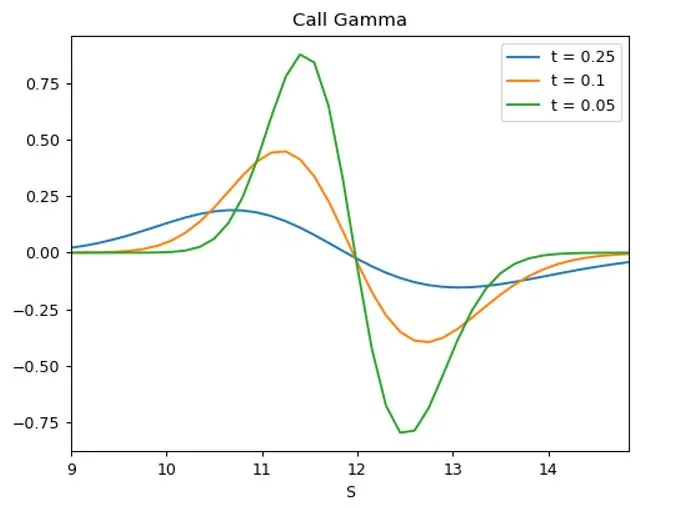
\includegraphics[width=\linewidth]{img/Exotic_Gamma.png}
\end{figure}

即便风险监控及时发现了风险,有时也很难进行对冲管理。

\subsection*{未使用适当的风险衡量标准}


\section*{FTX的崩塌}

